\chapter{Selection of Third Party Software}
\label{chapter:selection.of.third.party.software}

This chapter will first describe the ingredients in our prototype software
stack. Afterwards we'll account for the tools we've used while developing
this software stack.

Firstly one important aspect with the software used in our thesis work
\dash{}from operating system to third party libraries\dash{}is
that it should only consist of \term{open source}
\sidenote{
  \work{The Open Source Definition} \citep{osind} dictates the terms
  software needs to follow to be accepted as open source.
  Some call open source for \term{Free Software} and the term
  \term{Free/Libre/Open Source Software} have been used to reconcile
  these different wordings. We're pragmatics like others
  \citep[p.~8]{fogel05} and are not going into the political details of
  these terms and are going to describe such software as open source
  throughout this thesis.
}
software. In our experience it's
invaluable to have sources available for all involved software. If one
encounter abnormal behavior or bugs it's much easier to locate them when one
have sources available and one can trivially (depending on the complexity of
the problem) create a patch that sorts them out. One of the motivating factors
of open source contributors is the opportunity for other users to find and fix
failures and provide improvements on their code \citep[p.~87]{hippel05}.

It's also our experience that one can find third party software that fits
one's problem domain more easily if one chooses to use open source software
because of the vast availability of such software.
\citet{deshpande08} found that the availability of open source
code and projects had grown exponentially from January 1995 to December 2006.

Lastly it's of importance to keep the act of conducting science open so that
future researchers easily can discuss, falsify, and improve on previous
research. Software is often an essential part of computer science research and
\citet[p.~430]{kelty05} therefore argues that open source
is a property to strive for when conducting such research.

\section{Prototype Software Stack}

Based on the architectural decisions made in 
\chapterref{implementation} we'll now go on to make more fine-grained choices
of what specific third party software components to utilize in our prototype
application. We've decided to harness some of the seemingly best freely
available software components in this software stack. The issue of such code
reuse was introduced by \citet[\pp{138}{142}]{mcilroy68} when he voiced a need
for the software industry to become industrialized. His proposed technique for
enabling mass-production of software was to offer components\dash{}families
of program routines that can be used for any given job. These components
should be created in a way so that they can fit together as building blocks.
The developer should be able to treat these components as \term{black boxes}.%
\sidenote[-2]{
  In the field of electronics black boxes are used to describe electronic
  circuits with a fixed set of terminals where one is deliberately ignoring
  the internals of the circuit. Only the external properties of the circuit
  given by the electronic properties of its terminals are emphasized
  \citep[\p{171}]{wilson79}. Paralleling with computer science we can think of
  a component, module, object, or routine (electronic circuit) as being a
  black box when we're only concerned with its input and output
  characteristics trough its interface (terminals).
}

After object-oriented programming became the most popular
programming paradigm%
\sidenote[10]{
  According to \abbr{TIOBE}'s list of of
  how popular different programming languages are (based on the number of
  engineers using them, courses given for them, and third party vendors
  endorsing them) 65.463 percent of language use were object oriented
  \citep{tiobe08}.
  The languages counted towards object orientation were: Java, \abbr{PHP},
  C++, Perl, Python, C\#, Ruby, Delphi, JavaScript, D, FoxPro, Ada, and
  ColdFusion.
}
it's become commonplace to offer software components in the form of classes
and modules which easily can be integrated into a new software project.
As \prequote[\p{37}]{alahmad99}{puts it}{%
  code reuse is what object-orientation [is] all about in the first place}
Such libraries or frameworks ought to provide more efficient development,
higher code quality, and easier maintenance \citep[\p{12}]{stroustrup96}.
We're therefore leveraging several such freely available software components
in our prototype system. We'll first survey system components utilized
on the client-side and then those selected for the server-side implementation.


\subsection{Client-side}

\subsubsection{Platform}
\label{section:selection.stack.client.platform}

The platform for the clients is in essence a web browser. We are making
changes to a web page (more correctly the \abbr{DOM} of a web page)
after all. The web browser have to be explicitly chosen
to be one that readily supports scripting existing
web pages\dash{}a term often called \term{user scripting}.
The \project{Firefox}%
\sidenote[3]{
  Firefox is available at \url{http://www.mozilla.com/en-US/firefox}.
}
web browser was the first browser providing a
plug-in for handling such scripting of web pages and seems to have the most
mature implementation in our view. Since Firefox also is the
most adopted%
\sidenote[3]{
  Firefox was the second most used web browser in Ferbruary 2008
  only surpassed by Microsoft's Internet Explorer
  \citep{onestat08}.
}
cross-platform open source web browser the platform choice was quite easy.

Firefox provide user scripting trough the means of the
\project{Greasemonkey}%
\sidenote[3]{
  Greasemonkey is available at \url{http://www.greasespot.net}.
}
browser extension. Essentially all it provides is the ability for a user to
install a script which can manipulate the behavior and properties of an
existing web page using the \term{\abbr{DOM}}.%
\sidenote[3]{
  The \abbr{DOM} is a three of objects representing the hierarchical
  structure of nested tags (with text and attributes) in \abbr{HTML}
  documents \citep[\pp{307}{310}]{flanagan06}.
}
When a user have such a script for a specific web page installed its
instructions will be executed on the next visit to the given site, enabling
all kinds of modifications to the \abbr{DOM}.
Some have predicted that Greasemonkey could enable users to
finally \val{take back the Web}\dash{}making the decision of how a web page
behaves and what information it presents the choice of the user of a web page,
not the creator \citep[pp.~3--4.]{filman06}
Although most often used
for customizing the appearance of a given web site \citep[p.~39]{vitali06},
Greasemonkey can also be used for creating new navigational designs on the
\urort{} web site.

Although we've settled on the Firefox and Greasemonkey platform there is a
certain possibility that our implementation could work in other browsers
providing user scripting. The \project{Opera} browser provides user scripting
without any plugins,%
\sidenote[-3]{
  For more information see
  \url{http://www.opera.com/support/tutorials/userjs/examples}.
}
the \project{Safari} browser can handle user script with the
\project{GreaseKit}%
\sidenote{
  GreaseKit for Safari is located at \url{http://8-p.info/greasekit}.
}
plug-in. Our prototype user script would not work in the Opera browser since
it does not allow a \code{XMLHttpRequest} for another domain than what the
user script is currently running in. As described in
\sectionref{implementation.architecture,extending.different.domain}
this is an essential feature for our implementation. Recent versions of
GreaseKit removed the possibility for such kinds of requests to take place.
We're therefore left with Greasemonkey for Firefox as our only deployment
platform.

\subsubsection{Programming language}
\label{section:selection.stack.client.language}

The ability to programmatically alter behavior inside web browsers was first
introduced by \project{Netscape} in their 2.0 version of the web browser
with the same name. \project{JavaScript} was first intended to be a
lightweight scripting language for gluing together \abbr{HTML} and applets
written in the \project{Java} programming language \citep{netscape95}.%
\sidenote[-12]{
  Sun Microsystems, the creators of Java, had negotiated with
  Netscape about including it in their second major web browser release.
  The development of JavaScript, then called Mocha, was already
  underway and people inside Netscape wondered why one needed two
  languages.
  \postquote{eich08}{%
    The answer was that two languages were required to serve the two
    mostly-disjoint audiences in the programming ziggurat who most deserved
    dedicated programming languages: the component authors, who wrote in C++
    or (we hoped) Java; and the `scripters', amateur or pro, who would write
    code directly embedded in HTML}
}
Java applets never took off and JavaScript soon became the \latin{de facto}
standard for enabling behavior on the Web and was standardized as
\project{ECMAScript} in 1997 \citep{ecma99}.

Because of this we had no say in what programming language to use on the
client-side. That is not to say that JavaScript is a poor programming
language. Contradictory to its name, JavaScript bears few similarities to the
Java language.%
\sidenote{
  The name was more of a marketing decision when Netscape teamed up
  with Sun
  \citep[p.~2]{flanagan06}.
}
Despite its origins as a scripting language JavaScript is now considered
a full-featured modern programming language
\citedouble{p.~2}{flanagan06}{p.~3}{resig06} including object-orientation.

\subsubsection{Convenience library}

We decided to use a JavaScript library to make interactions with the
\abbr{DOM} simpler.
In addition there recent JavaScript convenience libraries provide a
unified interface to the browser\dash{}abstracting away inconsistencies
between browser vendors. Lately a myriad of such frameworks have appeared,
but the most interesting ones seems to be
\project{Prototype},
\project{Yahoo! UI Library} (\abbr{YUI} for short),
\project{MooTools},
\project{MochiKit}, and
\project{jQuery}.%
\sidenote[-2]{
  Available, in respective order, at
  \url{http://www.prototypejs.org},
  \url{http://developer.yahoo.com/yui},
  \url{http://mootools.net},
  \url{http://mochikit.com}, and
  \url{http://jquery.com}.
}
There are other frameworks available that provide everything but the kitchen
sink but we needed a lightweight or modular solution.

\begin{figure}
  \includegraphics{chart_javascript_size}
  \caption[JavaScript Library Comparison]{%
    Comparison of JavaScript library file size, in kB.
  }
  \label{figure:chart.javascript.size}
\end{figure}

As can be seen in
\figureref{chart.javascript.size}
we summarized the size of the most
current version for each library of this writing. These are not exact
metrics\dash{}we selected not to include certain widgets and logging
facilities for the modularized libraries\dash{}but should provide clear
guidance. To keep a level playing feel in this comparison we did not use
minified (removal of comments and unnecessary spaces) or packaged (compressed)
versions of the libraries. All comments and documentation was stripped with a
small script presented in \sourcecodepageref{javascript.comment.sripping}
since the in-line documentation and commenting varied amongst the libraries.

We played around a bit with the different libraries to get a feel for how
they worked. What follows is a comparison of simple \abbr{DOM} manipulation
for the different libraries. We followed the official documentation for the
various libraries and tried to solve or problem as succinct and clearly as
possible. We tried to add a \code{class} attribute of \val{highlight} to
all \code{em} elements with an descendant \code{p} element: 

\begin{scode}{Java}{dom.manipulation.prototype}{%
  \abbr{DOM} Manipulation with Prototype}{%
  \abbr{DOM} manipulation in JavaScript with the Prototype library}
\begin{lstlisting}
getElementsBySelector("p em").each(function(em) {
  em.addClassName("highlight");
});
\end{lstlisting}
\end{scode}

\begin{scode}{Java}{dom.manipulation.yui}{%
  \abbr{DOM} Manipulation with Yahoo! \abbr{UI} Library}{%
  \abbr{DOM} manipulation in JavaScript with the Yahoo! \abbr{UI} library}
\begin{lstlisting}
var em = YAHOO.util.Selector.query("p em"); 
YAHOO.util.Dom.setClass(em, "highlight);
\end{lstlisting}
\end{scode}

\begin{scode}{Java}{dom.manipulation.mootools}{%
  \abbr{DOM} Manipulation with MooTools}{%
  \abbr{DOM} manipulation in JavaScript with the MooTools library}
\begin{lstlisting}
$$("p em").each(function(em){
  em.addClass("highlight");
});
\end{lstlisting}
\end{scode}

\begin{scode}{Java}{dom.manipulation.mochikit}{%
  \abbr{DOM} Manipulation with MochiKit}{%
  \abbr{DOM} manipulation in JavaScript with the MochiKit library}
\begin{lstlisting}
var p = getElementsByTagAndClassName("p");
for (i = 0; i < p.length; i++) {
  em = getElementsByTagAndClassName("em","*", p[i]);
  for (j = 0; j < em.length; j++) {
    addElementClass(em, "highlight");
  }
}
\end{lstlisting}
\end{scode}

\begin{scode}{Java}{dom.manipulation.jquery}{%
  \abbr{DOM} Manipulation with jQuery}{%
  \abbr{DOM} manipulation in JavaScript with the jQuery library}
\begin{lstlisting}
$("p em").addClass("highlight");
\end{lstlisting}
\end{scode}

When we compare these rather trivial problem solutions it becomes apparent
that choosing a JavaScript library can have major impact on how easily
implemented and understood your code will be. Four of the five libraries
have support for selector syntax based on
that found in \abbr{CSS}.%
\sidenote{
  \abbr{CSS} is short for Cascading Style Sheets\dash{}a stylesheet language
  most commonly used for describing the presentation of \abbr{HTML} documents.
}
This is what makes the MochiKit example the most complex one, requiring the
developer to do two queries into the \abbr{DOM} and construct two
loop structures for iterating over the results.
Prototype and MooTools also requires the developer to loop over a single
result set, but the iteration is abstracted into an \code{each} function
making the logic a bit more clearer. Yahoo! \abbr{UI} Library's \abbr{DOM}
functions works on both single elements and collections of
elements\dash{}eliminating the need for an explicit loop structure.
Notice though that the library from
Yahoo! relies heavily on namespacing\dash{}which is a good thing for
interoperability with other libraries\dash{}but can be a bit verbose at times.

The solution written with jQuery provides even more clarity.
Every query into the \abbr{DOM} returns a special jQuery object which means
that one can call methods like \code{addClass} directly on this object
regardless if the jQuery object holds a single or multiple elements.
Also unique to jQuery is the fact that every method call returns a new jQuery
object. This means that one can \term{chain} methods together, expressing
succinctly and clearly what you intend to accomplish with your code. We can
extend our initial problem and add some punctuation inside our \code{em}
element:

\begin{scode}{Java}{jquery.method.chaining}{%
  jQuery Method Chaining}{%
  Chaining multiple methods together in jQuery}
\begin{lstlisting}
$("p em").addClass("highlight").append("!");
\end{lstlisting}
\end{scode}

Based on the minimal file size jQuery provided (only outbested by MooTools)
and its clear and unique syntax we decided on selecting it as the JavaScript
library for our implementation. It seems others have take jQuery and its
virtues to hart as many large corporations like Google, Intel, Dell, and
\abbr{BBC} have used it in their public facing offerings.%
\sidenote{
  For a complete list see \url{http://docs.jquery.com/Sites_Using_jQuery}.
}

\subsection{Server side}

\subsubsection{Platform}

Based on the following survey of server side software we needed an
\abbr{UNIX}-based operating sytem as the plattform of our server. The
particular operating system was pre-selected for us as \abbr{SINTEF} already
had a server we could use. This system was running \project{Debian}%
\sidenote{
  Debian \abbr{GNU}/Linux is freely available at \url{http://debian.org}.
}
\abbr{GNU}/Linux\dash{}a perfect fit for the rest of our server side
software stack.

\subsubsection{Programming language}
\label{section:selection.stack.server.language}

When doing prototype work it's important that the programming language one
uses is efficient to work with. This means that programmer efficiency is more
important than computational efficiency (a language's native performance).
\citet{mcanally08} argues that the true measure of a language's productivity
is how little code you need for solving a given problem.
Since we didn't have time to invest in learning a new language we had to do
with those we knew from before. Of those \project{Ruby},%
\sidenote[-7]{
  The Ruby language is available at \url{http://ruby-lang.org}.
}
\project{Python},%
\sidenote[-5]{
  The Python language can be found at \url{http://python.org}.
}
and \project{Common Lisp}%
\sidenote[-3]{
  Common Lisp, the prevalent Lisp dialect today, is a standard \citep{ansi96}
  and has many implementations.
  A gateway to this language and its many implementations can be found
  at \url{http://common-lisp.net}.
}
were the ones with language features that fitted our development process.
All these languages supports multiple programming-paradigms though Common
Lisp is most functional of nature  while Python and Ruby are more
inclined towards object-orientation.

They are all \term{latent typed}%
\sidenote[1]{
  Latent typing ``is a style of typing that does not require (or perhaps even
  offer) explicit type declarations''\citep{wikipedia08latent}.
}
and have quite expressive syntax. This makes for concise source code.
\citet{yegge07} argues that the worst thing that can happens to a code base is
size which often is the result of code bloat. In addition, both Ruby, Python,
and Common Lisp are \term{interpreted} languages.%
\sidenote[1]{
  This is only partly true since Common Lisp implementations incrementally
  compile code and extensions or new implementations for Python and Ruby
  implements just-in-time compilers. In both cases the developer
  does not need to explicitly invoke a compile process before using
  a program, therefore resembling interpreted languages.
}
This means that the programmer don't have to go trough a compilation process
before he can see the results of his labor. When prototyping rapidly it's
quite convenient to make small changes and see the results instantanously.

Disussion of the virtues of different flavors and implementations of
programming languages have been the subject of endless debate.
In the end we think it comes down to
personal preference and making a pragmatic choice for the tool best suited for
the job at hand. If we had to select a programming language based on our list
of candidates based on the languages syntax and posibilities in itself we
would probably have gone with Common Lisp. \citet[p.~27]{foderaro91} have
called it ``the programmable programming language''based on the fact that
program code in Lisp is data and can be manipulated with the same constructs
one are using on data. This makes it immensly powerfull and is the reason why
it's survived for over 50 years \citep[p.~217]{mccarthy78}
and been able to adopt new paradigms in programming as they've appered.
Even though we walue programming efficiency over computational performance,
it should be noted that Common Lisp have been described as the only performant
dynamic language \citep{martin08} compared to statically compiled languages.%
\sidenote[-8]{
  In \work{The Computer Language Benchmarks Game}
  (see \url{http://shootout.alioth.debian.org})
  several programming
  languages are pitched against each other in several tests to determine
  their computational performance. As of this writing (April 2, 2008)
  Common Lisp is 1.8 times slower than the fastest language: C++. Python
  and Ruby are respectively 18 and 56 times slower than the leader.
}

As it turns out, the most important criteria for choosing our implementation
language was its library support.

\begin{fullquote}{guo06}{shares this viewpoint:}
  The programming environment (development/target platforms, intended
  audience, and most importantly, available libraries) is the primary factor
  in determining one's choice of programming language.
\end{fullquote}

In the next section we discuss our options
of such libraries or frameworks. Based on our findings there we landed on
Ruby as the language of our server-side implementation.

\subsubsection{Data extraction library}

The core library we need is one that handles data extraction from existing
web pages, so called \abbr{HTML} \term{scraping}. While it's possible to
handle such problems with regular expressions, this becomes tedious after a
while. We therefore prefer a special purpose library.

The major deciding factor when we selected the implementation language was
the availability of such a library and its usefulness. We've already
revealed Ruby as our implementation language and are therefore killing the
suspense. Our data extraction library of choice is called \project{Hpricot}%
\sidenote[-4]{
  Hpricot can be obtained from \url{http://code.whytheluckystiff.net/hpricot}.
  A curious note: Hpricot is written by the same person who created
  Hoodwink.d\dash{}our inspiration for a transparent prototype implementation.
}
and makes \abbr{HTML} parsing a blissful endeavor in our opinion.

The Python alternative for web page scraping is \project{Beautiful Soup}.
We were not able to find any libraries specially made for \abbr{HTML} scraping
implemented in Common Lisp. There exists several \term{\abbr{XML}}%
\sidenote{
  Extensible Markup Language. General purpose markup language specification
  that enables implementors to create custom markup languages.
  \abbr{HTML} is not a subset (specified in) \abbr{XML} \citep{w3c99}.
  \term{\abbr{XHTML}} on the other hand, a reformulated version of
  \abbr{HTML}, is a subset of \abbr{XML} \citep{w3c02}.
}
libraries that could handle our tasks, but none as well integrated as
the Ruby and Python options.

To get a feel for the difference between Hpricot and Beautiful Soup we tried
them out on some trivial examples. Under you'll see the listings for one
of these examples. We are trying to find an \code{em} element with a class
of \code{citation}, which have a \code{p} element as its parent,
in a \abbr{HTML} document contained in the \code{html} object:

\begin{scode}{Python}{parsing.beautiful.soup}{%
  Parsing with Beautiful Soup}{%
  \abbr{HTML} parsing in Python with Beautiful Soup}
\begin{lstlisting}
html('p').content.findNextSiblings('em', 'citation')
\end{lstlisting}
\end{scode}

\begin{scode}{Ruby}{parsing.hpricot}{%
  Parsing with Hpricot}{%
  \abbr{HTML} parsing in Ruby with Hpricot}
\begin{lstlisting}
  html/'p > em.someclass'
\end{lstlisting}
\end{scode}

We feel that Hpricot's syntax is much clearer than that of Beautiful Soup.
This could be a personal preference since we've used \abbr{CSS} for a long
time and Hpricot's selector syntax is based on \abbr{CSS} and Xpath, just as
jQuery. Hpricot was in fact initially based on jQuery's selector syntax
\citep{why06}. This means that we can use the same syntax for selectors on the
server and client-side\emph{}a cognitive advantage.

When we started developing our prototype application we came over what in
some way can be seen as a bug of Hpricot. We feel the fault lies
with the server-side plattform \urort{} uses. Simply put, Microsoft's
\project{ASP.NET} web application framework uses a hidden \abbr{HTML}
input element to maintain the state of \abbr{HTML} forms between
stateless \abbr{HTTP} requests. This hidden input element can be quite large%
\sidenote{
  On the \urort{} web site
  (\url{http://www11.nrk.no/urort/Artist/dividizzlDVD})
  the hidden input element used for maintaining state weighted in at 122kB!
}
in size since it contains a serialized version of the state of the current
page's \abbr{HTML} forms. Such large single \abbr{HTML} elements have been
described by Microsoft itself as a problem \citep{mitchell04}.
Hpricot sets aside a buffer of 16kB for storing each \abbr{HTML} element.
When Hpricot encounters an element with the size we're seeing on \urort{}
it simply chokes.

Since Hpricot is open source software someone had thankfully experienced
the same problem and provided a patch to dynamically increase the
buffer if an enormous \abbr{HTML} element was encountered. All we had to do
for properly using Hpricot on \urort{} was to use a version patched with this
change instead of using the standard vanilla version.

\subsubsection{Data fetching library}

Since we've selected Ruby as our development language of choice we used
\executable{open-uri}, part of the standard Ruby library, for fetching
documents over \abbr{HTTP}.
\executable{open-uri} is trvial to use and integrates nicely with Hpricot:

\begin{scode}{Ruby}{fetching.openuri.parsing.hpricot}{%
  Fetching and Parsing with Hpricot and open-uri}{%
  Fetching a \abbr{HTML} document with \executable{open-uri}
  and parsing it with Hpricot to find the first and
  last name of a hCard Microformat}
\begin{lstlisting}
require 'hpricot'
require 'open-uri'

html = Hpricot(open('http://redflavor.com'))
(html/'address.vcard > .fn').inner_html
# => "Eivind Uggedal"
\end{lstlisting}
\end{scode}

\subsubsection{\abbr{JSON} library}

Since we'll mainly be serving requests
for our JavaScript based client implementation we found it sound to transfer
this data as \abbr{JSON}.%
\sidenote[-1]{
  \abbr{JSON}, short for JavaScript Object Notation, is specified in
  \abbr{RFC} 4627 \citep{crockford06b}. Shortly put it's a lightweigh data
  interchange format based on the object literals of JavaScript.
}
Luckily for us there exists a libary for encoding
Ruby objects into \abbr{JSON} format
simply called \project{json}.%
\sidenote[3]{
  The Ruby \abbr{JSON} can be found at \url{http://json.rubyforge.org}.
}
The next code listings show how simple objects can be encoded and the
resulting \abbr{JSON} format.

\begin{scode}{Ruby}{json.encoding}{%
  Encoding to \abbr{JSON}}{%
  Encoding a Ruby hash to \abbr{JSON} format}
\begin{lstlisting}
msg = {:interjection => 'hello',
       :noun         => 'world',
       :suffix       => '!'}

msg.to_json
\end{lstlisting}
\end{scode}

\begin{scode}{Java}{json.result}{%
  Result of \abbr{JSON} Encoding}{%
  The result of the \abbr{JSON} encoding of a Ruby hash}
\begin{lstlisting}
{"interjection": "hello",
 "noun":         "world",
 "suffix":       "!"}
\end{lstlisting}
\end{scode}

\subsubsection{\abbr{HTTP} framework}

A web framework or rather \abbr{HTTP} framework is needed to make the
generated activity data in \abbr{JSON} format available for our client.
In addition we need to provide some traditional \abbr{HTML} pages and
take action on input we receive from some of these.

There is numerous frameworks for easing the creation of \abbr{HTTP}
applications available for Ruby. The most popular%
\sidenote[-1]{
  A search for Ruby on Rails books on Amazon revealed 35 titles as of
  20 May, 2008.
}
is \project{Ruby on Rails}.%
\sidenote[2]{
  Ruby on Rails has its home at \url{http://rubyonrails.org}.
}
Other actively developed frameworks include
\project{Merb},
\project{Camping},
\project{Sinatra}, and
\project{Ramaze}.%
\sidenote[2]{
  Available at
  \url{http://merbivore.com},
  \url{http://code.whytheluckystiff.net/camping},
  \url{http://sinatrarb.com}, and
  \url{http://ramaze.net} respectively.
}
These frameworks have a varying degree of complexity, but none of them
is as simple as \project{Rack},%
\sidenote[6]{
  Rack is available at \url{http://rack.rubyforge.org}.
}
a web server interface that sits between a web framework and a web
server or can be used as a very light weight web framework on its own.
Since we our neeeds were a bit specialized we decided to use Rack for
handeling \abbr{HTTP} requests. Because of its simplicity it's very
flexible and allowed us to create exactly the \abbr{HTTP} interface
we wanted. By using Rack we can also easily swap between different
web servers that support the protocoll mandated by Rack's interface layer.

\subsubsection{\abbr{HTTP} server}

Since our web framework builds on Rack we have several
\abbr{HTTP} servers to select from. The most prominent alternatives
of Ruby servers are%
\sidenote{
  These servers can be found at respectively
  \url{http://webrick.org},
  \url{http://fastcgi.com},
  \url{http://mongrel.rubyforge.org}.
  \url{http://swiftiply.swiftcore.org/mongrel.html},
  \url{http://code.macournoyer.com/thin}, and
  \url{http://ebb.rubyforge.org}.
}:

\begin{items}
  \iterm{Webrick} is the original Ruby web server included in all recent
    versions of the Ruby environment. Because of its simplicity it has
    been widely used when developingweb applications. Unfortunately it's
    painstakingly slow compared to the other alternatives.
  \iterm{FastCGI} was the de facto way of running Ruby web applications
    for production systems before Mongrel, the following alternative,
    was released. It's basically an improvment over the well known
    \abbr{CGI} model. Contrasted to its ancestor the processes
    of FastCGI are persistent and are reused when handeling requests
    \citep{openmarket96}.
  \iterm{Mongrel} was introduced as a faster alternative to Webrick.
    One of the distinguishing factors of the library is that it
    handles each request in its own thread\dash{}enabeling it to
    handle many concurrent requests. The project is now very mature
    and can be concidered as the most stable Ruby web server.
  \iterm{Evented Mongrel} is a fork of Mongrel which uses
    an event loop using the Reactor pattern
    \citep[\p{529}]{schmidt95}
    instead of using threading to handle multiple concurrent requests.
    The requests are therefore handeled sequentially.
  \iterm{Thin} is a fork of Evented Mongrel, promising even better
    performance than the original Mongrel. It's an sequential
    server which includes various
    convenience functions for easily starting, stopping, and managing
    a wide array of Thin servers.
  \iterm{Ebb} is the newest kid on the block and are proving to be
    faster than its predecessors. It's entrirely written in C
    and uses C libraries in contrast to Mongrel and the Mongrel forks
    which are only partly written in C with Ruby libraries.
    It supports both sequential and threaded processing of requests.
    This project is fairly new and it's not recommended to utelize it
    in production yet.
\end{items}

As we've seen the Ruby web server offerings are many and it can be quite hard
to find out the best option. We first and foremost wanted a stable solution
with decent performance. This eliminated Ebb in spite of its promising
performance characteristics. Webrick and FastCGI is fairly outdated and leaves
something to be desired in the performance department. Thin seems to have
taken over the space Evented Mongrel used to occupy in the Ruby server world
because of its ease of use and improved performance.

This leaves us with two choices: Thin and Mongrel. The most distinguishing
feature between them is that Thin processes requests sequentially and Mongrel
processes them in threads, enabeling concurrent processing. Wether
sequential or concurrent processing is best depends on your application.
In general a concurrent model wins when you have varying response times.
If for instance one request takes several seconds to process all other
requests to you application have to wait until the first request have
finished processing when one are using a sequential model. For a concurrent
model the first request can be processed in its own thread while new requests
can be accepted and processed in their own threads.

Why then not use a concurrent model all the time? The drawback with a
cuncurrent model is that creating threads is costly and introduces some
overhead\dash{}resulting in longer response times. If your application
only have fairly short response times you can take advantage of a
sequential model where the time to process a response will be lower compared
to a scenario where one have to create a new thread for each request.

\citet{zygmuntowicz08} recommends using Mongrel, the concurrent server,
for general purpose applications. He goes on to say that the treshold
for wether one should use a sequential server is response times that
are no longer than 2--3 seconds. Seeing as our application could very
well fall outside this treshold for some requests%
\sidenote[-5]{
  When the data the user is requesting can not be found in the cache
  we have to retrieve the data from \urort{} and perform calculations
  on it. This can be quite time consuming and could very well exceed
  the 2--3 second treshold \citeauthor{zygmuntowicz08} recommends
  to use as guidance in server selection.
}
we followed the recommendations from \citeauthor{zygmuntowicz08} an opted
to use Mongrel as our Ruby web server. By doing so we're on the safe side
and can deliver simultaneous requests even if one of the requests are taking
overly long to process. In addition we believe the overhead of using a
concurrent model with threading would not introduce to much delay in
response time for average timed requests compared to a sequential model.

\subsubsection{Cache library}
\label{section:selection.stack.server.cache}

As detailed in \sectionref{implementation.architecture.caching} we had no need
to persist our activity data since it was changing as time went by. We did
however want to cache this data for a given time so that users would get
berable request times when using our prototype implementation.

We did not test various cache solutions but instead went with a proven
cache solution called \project{Memcached}.%
\sidenote[-3]{
  Available at \url{http://www.danga.com/memcached/}.
}
Memcached was developed at \project{LiveJournal}%
\sidenote[-2]{
  LiveJournal is a place where people can keep a blog or journal with
  some social network features baked in. As of May 20, 2008 LiveJournal
  had over 15 million registered users \citep{livejournal08}. LiveJournal is
  available at \url{http://livejournal.com}.
}
to handle caching of data for their large user base. Memcached is used by many
large web sites and Facebook is currently the largest user of the
caching solution \citep{facebook08b}. Memcached is very performant since it
stores all its cached items in memory. To interact with the Memcached server
we used the \project{memcache-client}%
\sidenote{
  Available at \url{http://seattlerb.rubyforge.org/memcache-client/}.
}
Ruby library.

\subsubsection{Database}

Since we were going to only use a single database table
(see \sectionref{implementation.architecture.code.structuring} for details)
and did not need any special features, we could
basically have used all freely avaiable relational database systems. We
selected \project{Sqlite}%
\sidenote[-1]{
  Available at \url{http://sqlite.org}.
}
as it have a much smaller footprint than it's
competitors. This is mainly due to it's limited featureset. Another usefull
characteristic of Sqlite is it's storage format. Sqlite simply writes to a
normal disk file that can be backed up and handeled with normal
file system tools.

For accessing the database we had a choice between several libraries that
makes interaction with the database easier and abstracted based on database
software.
We selected the library we found had the most flexible and lightweight
\abbr{ORM} capability: \project{Sequel}.%
\sidenote{
  Sequel have a home at \url{http://sequel.rubyforge.org}.
}

\subsection{Overview of client \oldand server components}

With all the pieces in place of our third party software puzzle
we present a high level view of the architecture, from the client to the
server, in
\figureref{fig.prototype.architecture}.
\tableref{third.party.software.versions} lists the versions we used of the
various third party software.

\begin{figure}
  \begin{whole}
    \includegraphics{fig_prototype_architecture}
    \caption[Prototype Architecture]{
      High level view of the overall prototype architecture.
    }
    \label{figure:fig.prototype.architecture}
  \end{whole}
\end{figure}

\begin{table}
  \begin{whole}
    \begin{tabular}{lll}

      & Name & Version \\

      \cmidrule(lr){2-2}
      \cmidrule(lr){3-3}

      Web browser &
      Firefox &
      User dependant (tested on 2.0.0.14 and 3.0 \abbr{RC}1) \\

      Client-side language &
      JavaScript &
      Browser dependant (tested on 1.7 and 1.8) \\

      User script extension &
      Greasemonkey &
      User dependant (tested on 0.7.20080121.0) \\

      JavaScript library &
      jQuery &
      1.2.4 \\

      Server-side plattform &
      Debian \abbr{GNU}/Linux &
      4.0 \\

      Server-side language &
      Ruby &
      1.8.5 \\

      \abbr{HTML} scraping library &
      Hpricot &
      0.6 (with buffer overflow patch) \\

      \abbr{HTTP} fetching library &
      open-uri &
      1.8.5 (included with Ruby) \\

      \abbr{JSON} library &
      json &
      1.1.2 \\

      \abbr{HTTP} framework &
      Rack &
      0.3.0 \\

      \abbr{HTTP} server &
      Mongrel &
      1.1.4 \\

      Cache server &
      Memcached &
      1.1.12 \\

      Cache access library &
      memcache-client &
      1.5.0 \\

      Database server &
      Sqlite &
      3.3.8 \\

      Database access library &
      Sequel &
      1.5.1 \\

    \end{tabular}
    \caption[Third Party Software Versions]{%
             Versions of third party software used
             in the prototype stack, by type}
    \label{table:third.party.software.versions}
  \end{whole}
\end{table}


\section{Development Tools}

As with the implementation platforms, languages, and third party libraries
our first criterion for selecting development tools is freedom.

\subsection{Version control}

We've found it indispensable to use \term{version control} when writing code
and even used it when authoring this thesis. We'll not spend time to discuss
the merits of version control since we feel its benefits are major and
using one induces almost zero overhead in your working process. Sometimes we
feel that the use of version control can guide you when conducting complex
tasks.

There are however several different forms of version control system one can
use. One of the most used version control implementations the last years
in open source circles was
\project{Subversion}%
\sidenote[-8]{
  Available at \url{http://subversion.tigris.org}.
}\dash{}a \term{centralized version control system} meaning that one central
server holds the version controlled code repository and its history.%
\sidenote[-8]{
  Developers on the client-side have working copies and need to contact the
  centralized server to get a hold of historical data and create new history.
}
Recently \term{decentralized version control systems} have become more popular
amongst developers. A decentralized model means that every developer can have
their own repository consisting of all history.%
\sidenote[-6]{
  You can for instance be without internet connectivity and still commit
  changes, revert to previous versions, and handle all other tasks your
  version control system supports.
}
Code is then shared either in a push or pull fashion between such individual
repositories. This enables a much better model for collaboration.
We favor this last model of version control and so have projects
like \project{Linux}, \project{X}, \project{Mozilla},
and \project{OpenSolaris}.%
\sidenote[-3]{
  \citeauthor{torvalds07}, author of the Linux kernel,
  have described Subversion and centralized version control
  as fundamentally flawed since it's supposed to be a
  \q{\abbr{CVS} done right}. Since he feels \abbr{CVS} is flawed Subversion
  is therefore inherently flawed \citeyearpar{torvalds07}.
}

Based on criteria of performance and current adoption there are in our view
only two interesting decentralized version control systems:
\project{Git}%
\sidenote[1]{
  Available at \url{http://git.or.cz}.
}
and \project{Mercurial}.%
\sidenote[3]{
  Available at \url{http://www.selenic.com/mercurial}.
}
Both are unique in that they don't track meta-data, they just track
content and meta-data are thereby inferred from the content.
At a very high level view Mercurial have a better user interface and Git
supports some advanced features the former don't have. We opted to used
Mercurial for this development project since we've substantial experience in
using it and did not need any of Git's advanced features.

\subsection{Editor}

A developer's main tool for authoring software is his editor. Sometimes the
language of implementation warrants a specialized editor with aids for
handling cumbersome tasks specific to that language. Such an editor is often
called an \abbr{IDE}%
\sidenote[-3]{
  A good example of an \abbr{IDE} (integrated development environment
  for short) is \project{Eclipse} (available at \url{http://eclipse.org}).
  It was first used for Java development but since extended with
  plugins for handling other programming languages and families.
}
and are used most often for languages like Java and C\#.
\citet{murphy06} found that developers mostly use an \abbr{IDE} for navigating
large collections of source code, refactoring code, debugging code, and
interacting with revision control systems in addition to normal editor usage.
Development environments found in Lisp%
\sidenote[1]{
  \prequote[\p{69}]{sandewall78}{%
    describes the nature and benefits of the Lisp environment as}{%
      The `residential' design of programing systems, whereby all facilities
      for the user are integrated into one system with which the user
      communicates during the entire interactive session, offers great
      possibilities for user convenience}
}
and Smalltalk%
\sidenote[9]{
  Similar to Lisp's programming environment
  \postquote[\p{viii}]{goldberg83}{%
    Smalltalk is designed so that every component in the system that is
    accessible to the user can be presented in a meaningful way for
    observation and manipulation}
}
are surpassing \abbr{IDE} types in integration and interactiveness even though
they preceded them.

The programming languages we previously settled on, JavaScript and Ruby,
are very expressive and dynamic in their nature in addition to being
interpreted instead of compiled. Our experience is that \abbr{IDE} usage for
such languages stands more in the way than aid you as a programmer during
your problem solving process.
\citet{bray07} conducted a rather unscientific survey of 1000 Ruby
programmers. Despite of the surveys shortcomings it showed that
the majority of Ruby programmers used non-\abbr{IDE} editors for their
development.

The interactive experience provided by Lisp and Smalltalk implementations are
sadly missing%
\sidenote[5]{
  Ruby has an interactive interpreter similar to those found in Lisp and
  Smalltalk environments called \executable{irb}. It's not integrated into an
  overall programming environment and therefore is mostly used for testing out
  small ideas.
}
from JavaScript and Ruby implementations. This means that we're left with
finding a good editor which enables us to focus on writing code as efficiently
and safely as possible. Editor selection is highly a matter of preference and
finding one that matches your work process. Powerful editors have a
reputation of being quite hard to learn. But if you get over the steep
learning curve the benefits the editor gives you are worth it.

\begin{fullquote}{orenstein08}{%
  have experienced how much effort programmers can
  invest in something seemingly trivial as an editor}
    If the thought of switching editors doesn't fill you with quite a bit of
    dread, what you're using now is almost certainly under powered, and you
    definitely haven't customized it enough.
\end{fullquote}

\subsection{Testing suites}

As described in \sectionref{implementation.process.testing} we're firm
believers of using automated testing when developing applications.

Greasemonkey user scripts inherit a strict security model where the
\abbr{DOM} one is interacting with are a special copy of the browser's
\abbr{DOM}. In the case of testing this is unfortunate since it's very
complicated to get a testing library to properly run within this secure model.

We initially tried to adapt the \project{Screw Unit}%
\sidenote{
  Screw Unit is available at \url{http://github.com/nkallen/screw-unit}.
}
JavaScript behaviour-driven development library to the intricacies of
Greasemonkey user scripts, but had to give up. We therefore had to develop
without automated tests on the client-side.
Fortunately the most complicated logic of our application are on the server
side and our client-side development process did not get to hard despite the
lack of a proper testing suite.

On the server-side we had better success with integrating a testing suite into
our application. There are several options available when selecting amongst
Ruby testing suites. We're ignoring traditional test-driven libraries as
we're proponents of a behaviour-driven style
(\sectionref{implementation.process.testing}). We looked at%
\sidenote{
  These behaviour libraries can be found at respectively
  \url{http://rspec.info},
  \url{http://rubyspec.org},
  \url{http://chneukirchen.org/repos/testspec}, and
  \url{http://chneukirchen.org/repos/bacon}.
}:

\begin{items}
  \iterm{RSpec} is the original behaviour-driven suite for Ruby. It's
    therefore the most mature project and have the best integration with
    other tools. It does seem to suffer from too much complexity in its code
    base. The following suties adresses this complexity problem.
  \iterm{MSpec} have more features than RSpec in spite of having clearer
    and more understandable source code \citep{klishin08}.
  \iterm{test/spec} is an interface for writing specifications of behavior
    on top of the original Ruby unit testing library and are therefore
    compatible with tests written with it.
  \iterm{Bacon} is the smallest of the suites when counting source code
    but still implements the majority of the fatures of its big brothers.
    It's still a young project and have therefore not seen much usage.
\end{items}

Based on the tool support and code maturety we decided to use RSpec for our
development. This allowed us to use \project{autotest}, a part of
\project{ZenTest}%
\sidenote{
  Available at \url{http://www.zenspider.com/ZSS/Products/ZenTest/}.
}
which continously runs your test suite as you make changes to your source code
files. This way you can keep your focus on the editor and only glance over the
status of your test suite as you move along.

\subsection{Debugger \oldand profiler}

Since we were unable to utilize automated tests on the client-side we had to
resort to a debugger checking for correctness in our code while developing.
There are currently two JavaScript debuggers for the Firefox browser:
\project{Venkman}%
\sidenote{
  Located at \url{http://www.mozilla.org/projects/venkman/}.
}
and \project{Firebug}.%
\sidenote[2]{
  Firebug has its home at \url{http://www.getfirebug.com}.
}
The latter have a considerably less intrusive interface than the former and
seems to be much more actively developed as of this writing. Firebug have the
most advanced features with a better user interface. Our choice of a client
side debugger was simple.

On the server-side we never saw the need for a debugger since we developed all
our code in a behaviour-driven way enabeling us to both catch bugs and form
solutions trough our specification suite. But as described in
\sectionref{implementation.performance} we stumbled upon some major
performance problems. For locating the bottlenecks in our
application\dash{}the places that consumed the most time\dash{}we used
a \term{profiler}%
\sidenote{
  A profiler is a tool used by developers for identifying the execution time
  of various parts of a program or how often these parts of the program are
  utilized \citep[\p{120}]{graham82}. It's used when trying to improve the
  performance of a segment of a given program and should be used in an
  iterative way \citep[\p{125}]{graham82}.
}
called \project{ruby-prof}.%
\sidenote[9]{
  Available at \url{http://rubyforge.org/projects/ruby-prof}.
}
This is the fastest profiler for Ruby and it can generate various forms of
reports which enables a developer to understand the time related aspects of
his code.
